\section{Evaluation} \label{sec:expr}
We implemented \tool based on Minisat v2.1.1, using C++. \tool, \ctool and \bc use the Minisat Solver as an oracle while \nbc and \bdd change the implementation of Minisat according to the algorithms.

The experiments are conducted on clusters with 64GB memory limitation and 10 hours runtime limitation. 
The operating systems are Red-Hat Enterprise Linux. We can not guarantee that the performances of CPUs in the cluster are exactly the same, thus all experiments are repeated 3 times and the average results are computed to enhance fairness. \tool runs sequentially in the experiments and does not use the incremental features in the Minisat Solver.

We use formulas from industrial tracks of SAT competitions from 2011 to 2017 as benchmarks. There are 1816 formulas in total, 552 of them are known as unsatisfiable, 608 of them are satisfiable and the satisfiability of the rest remain unknown. Therefore, the size of the final benchmark is 608. The origin of these formulas includes encryption problems, planning problems, hardware model checking problems and fault localization problems, etc.

\subsection{Overall Performance of the Tools}
Table \ref{tab:main} shows the overall performance of the tools. The first column of Table \ref{tab:main} is the name and the number of the formulas. For clarification, we only include the formulas that at least one of the tools solves them. The second column is the average number of variables, and the third column is the average number of clauses of the formulas. The forth column is the average number of solutions in the formulas. Starting from the fifth column, the number of formulas solve by \tool, \ctool, \bc, \nbc and \bdd are listed respectively.
There are 79 formulas that are solved by at least one of the tools. \tool solves all 79 formulas, \ctool solves 65 formulas, \bc solves 64 formulas, \nbc solves 53 formulas and \bdd solves 51 formulas. For the other 4 comparing tools (\ctool, \bc, \nbc and \bdd), there exists at least one group of formulas that the tools only solve a small part of them. For example, \nbc only solves 1 formula in the Dimacs group, and \ctool failed to solve a formula in the Complete group.
\tool solves the most formulas among the 5 tools, which indicates that the efficiency of \tool is better than the comparing tools with the given benchmark.

\begin{table*}
\begin{tabular}{cccccccccc}
\toprule
Formulas & AveVAR & AveCL & AveFST & \#AveSATInst & \tool & \ctool & \bc & \nbc & \bdd \\
\midrule
Dimacs(15) & 680 & 17079 & 508.14 & 1 & 15 & 15 & 13 & 1 & 15 \\
AProve(2) & 8565 & 28931 & 7.32 & 78 & 2 & 2 & 2 & 2 & 2 \\
Complete(4) & 600 & 27140 & 0.02 & 1 & 4 & 0 & 4 & 4 & 0 \\
Encryption(12) &  8616 & 82773 & 44.75 & 1 & 12 & 10 & 12 & 11 & 6 \\
Manthey(24) & 5179 & 23692 & 780 & 2.58 & 24 & 18 & 14 & 21 & 16 \\
Mp1(12) & 16301 & 185948 & 630.41 & 305.75 & 12 & 11 & 12 & 9 & 8 \\
Others(10) & 11593 & 44557 & 325.19 & 1131 & 10 & 9 & 7 & 5 & 4 \\
Total(79) & 7323 & 393119 & 327.97 & 227.79 & 79 & 65 & 64 & 53 & 51 \\
\bottomrule
\end{tabular}
    \caption{Overall Performance of ALLSAT Computing Tools}
    \label{tab:main}
\end{table*} 

For the 31 formulas that are solved by all the 5 tools, \tool uses the least computing time (9558.64 seconds), which is 51\% less than \ctool (19427.51 seconds), 48\% less than \bc (18221,86 seconds),  54\% less than \nbc (21263.27 seconds) and 67\% less than \bdd (28901.35 seconds).
Since only \tool solves all the 79 formulas, we only compare the computing time among the formulas that are solved by both \tool and one of the comparing tools (including \ctool, \bc, \nbc, and \bdd).

There are 65 formulas solved by both \tool and \ctool, \ctool uses less computing time than \tool for 11 of the formulas, for the rest 54 formulas, \tool uses less computing time. In total, \tool uses 86274.54 seconds and \ctool uses 110932.01 seconds, which is 22\% more than \tool uses.
There are 64 formulas solved by both \tool and \bc, \bc uses less computing time than \tool for 22 of the formulas, for the rest 44 formulas, \tool uses less computing time. In total, \tool uses 92198.9 seconds and \bc uses 110932.01 seconds, which is 37\% more than \tool uses.
There are 53 formulas solved by both \tool and \nbc, \nbc uses less computing time than \tool for 20 of the formulas, for the rest 33 formulas, \tool uses less computing time. In total, \tool uses 28024.15 seconds and \nbc uses 123761.88 seconds, which is 78\% more than \tool uses.
There are 51 formulas solved by \tool of \bdd, \bdd uses less computing time than \tool for 9 of the formulas, for the rest 42 formulas, \tool uses less computing time. In total, \tool uses 74686.244 seconds and \bdd uses 107023.29 seconds, which is 31\% more than \tool uses.

Based on the comparison of number of solved formulas and computing time between \tool and the other comparing tools, we conclude that \tool is able to solve the most formulas with the least computing time, and \ctool ranks the second place in the comparison. 
\bc solved the third most number of formulas.
The \nbc and \bdd tools solve less formulas with more computing time. 
It indicates that for formulas from the industrial benchmark, blocking based tools have advantages than non-blocking based strategies and BDD based strategies.
We then compare the performance of blocking based tools, including \tool, \ctool and \bc.

\subsection{Compassion among Blocking based Tools}

\begin{figure}
    \centering
    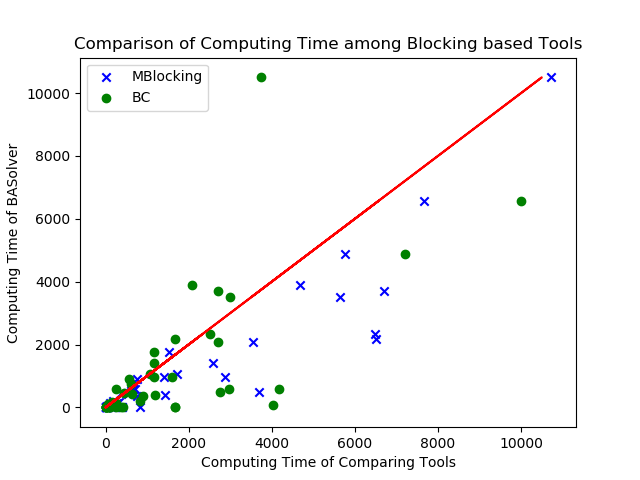
\includegraphics[scale=0.5]{allsat-time.png}
    \caption{Comparison of Computing Time between \tool and Other Tools}
    \label{fig:allsat-time}
\end{figure}

There are 53 formulas that are solved by all the the three tools. Figure \ref{fig:allsat-time} shows the computing time comparison among the 53 formulas. The x-axis is the computing time of the comparing tools, and the y-axis is the computing time of \tool. The line (red) is the base line, set up by the computing time of \tool, the circles (green) are the comparing data of \bc, the crosses (blue) are the computing data of \ctool. For the circles and crosses that are above the line, the computing time of the comparing tools are less than \tool. Results show that for the majority of the formulas, \tool needs less computing time than both \ctool and \bc. And \ctool needs more computing time than \bc on general. It is because that \bc only uses the decision variables in the blocking clauses, therefore, the blocking clauses of \bc is shorter than \ctool. 

Figure \ref{fig:allsat-blk} shows the length of blocking clauses of the three tools. The x-axis is the length of blocking clauses in \ctool and \bc, and the y-axis is the length of blocking clauses in \tool. The line (red) is the base line set up by the length of blocking clauses in \tool, the circles (green) are the comparing data in \bc, and the crosses (blue) are the comparing data in \ctool. The scatter only shows the formulas which average length of blocking clauses is less than 2000. From Figure \ref{fig:allsat-blk}, we can see that for most of the formulas, the length of average blocking clauses in \tool is shorter than \ctool and \bc, which is an important reason that \tool uses less computing time than \ctool and \bc.

With the results of Figure \ref{fig:allsat-time} and \ref{fig:allsat-blk}, we observe that tools with shorter blocking clauses perform better than the ones with longer blocking clauses.
The average length of blocking clauses in \tool is 1026 (among the 79 formulas), the average length of blocking clauses in \ctool is 22182 (among the 65 formulas) and the average length of blocking clauses in \bc is 6180 (among the 64 formulas).
The reason for \tool with short length of blocking clauses is because by using backbone information, a huge part of variables are removed from the blocking clauses. Therefore, backbone information contributes to the computing of ALLSAT problems.

\begin{figure}
    \centering
    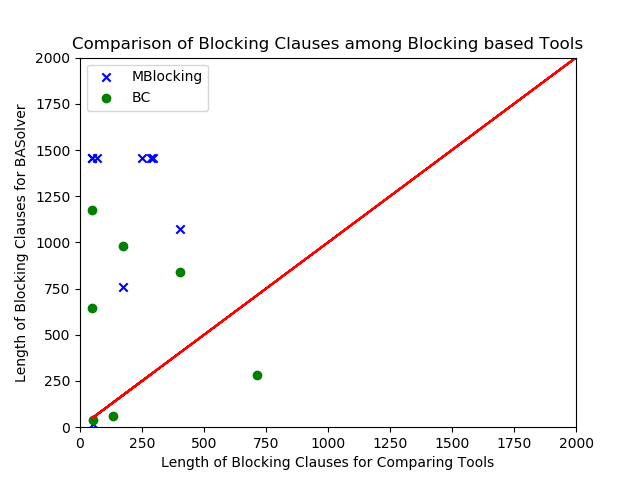
\includegraphics[scale=0.5]{allsat-blk.png}
    \caption{Comparison of Length of Blocking Clauses between \tool and Other Tools}
    \label{fig:allsat-blk}
\end{figure}

%i st bb
% 27.32,34.43,168.48,387.22,953.46,890.8,1406.37,3881.49,5080.45,3508.42,3705.65,6577.17,4876.69,0.02,22.02,9.82,592.7,0.02,592.02,8.81,44.91,59.41,134.19,18.56,112.81,51.46,44.58,18.56,143.73,71.98,51.46,0,0,0.05,2190.72,214.49,494.58,41.27,28.4,421.93,1059.84,2324.63,348.22,967.44,2085.02,5.17,581.39,1777.66,750.19,461.1,12.52,6.33,15.55

% i st blocking
% 50.724706,85.540464,328.695662,1431.727754,2885.069117,746.469704,2585.627846,4692.450813,10711.73746,5651.043807,6709.192745,7665.512216,5760.008729,0.044148,32.382529,11.55542,648.974382,0.143299,697.239595,397.705001,62.550608,130.845185,275.502498,230.81965,262.200193,42.852047,208.340364,25.225832,99.69934,161.046904,172.878436,0.00411,0.010488,0.081907,6499.114935,190.740354,3684.199977,83.985681,133.480907,537.683497,1722.517,6487.315428,764.011712,1406.584865,3547.320029,37.498138,658.131014,1539.000674,604.946888,374.969432,154.215404,385.291636,829.254055

% i st bc
% 75.73,60.59,158.33,1189.73,1171.08,560.48,1165.73,2081.53,3738.13,2989.81,2709.9,10005.95,7206.26,0.01,104.28,57.2,245.39,0.04,2981.58,360.28,48.64,75.24,158.93,18.02,63.37,241.44,59.02,247.22,261.27,4026.74,27.7,0,0,0.08,1680.67,839.03,2756.77,41.02,1665.14,630.75,1062.46,2524.73,913.3,1595.89,2706.84,55.84,4174.49,1177.78,615.5,440.08,107.67,418.03,1665.82

% blk bb
% 54,3069,714,403,132,69184.8,48,248.619256,284.5,66.85714286,48,294.4743802,173.25

% blk bc
% 41,2061,285,841,62,2210,643,31933,299335,15284,1173,56597,979

% blk blocking
% 19,8567,8564,1075,3842,11520,1458,1458,1458,1458,1458,1458,760



